\newpage

\section{Internal Software}

The in this section described processes are internal processes, i.e. running on the robot itself. In total there are three custom processes running on the robot. Figure \ref{fig:software} shows the structure of the developed software. This section focuses on the base and the navigation process. The image streaming process is referenced in section \ref{sec:image_processing}.

\begin{figure}[H]
\centering
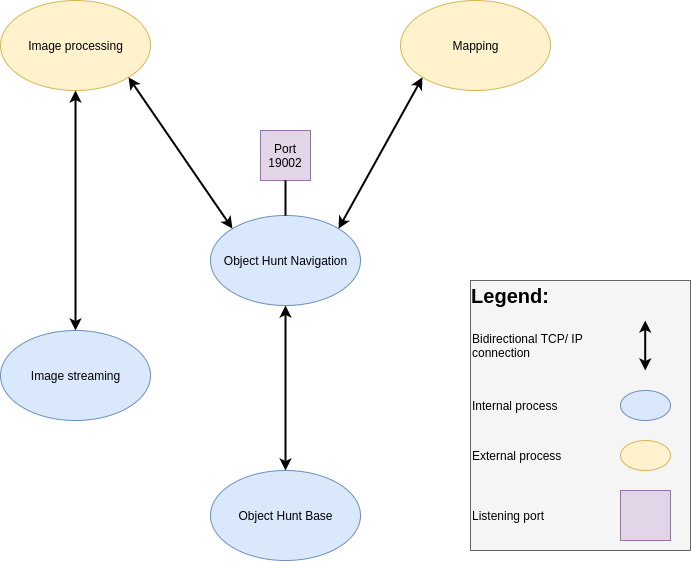
\includegraphics[scale=0.6]{sources/software_structure.png}
\caption[Software structure]{Software structure}
\label{fig:software}
\end{figure}

\subsection{Design Principles}

The system in its entirety shall not be bound to any programming language. In that way virtually any language that supports the usage of raw sockets in collaboration with TCP/\,IP can be used to develop software for the system. At the time of writing this report Java, Python and C++ are already employed.\\

Furthermore underlies the internal software particular specifications, which are defined at the beginning of the project. They define, among other things, how the system as a whole will behave and handle dedicated tasks, i.e. inter-process communication. The compliance of these principles ensure that the developed software works in the expected manner and offers the possibility for adding further processes in the future.\\

The defined principles are listed in the following:

The internal software underlies software specifications, which are defined at the beginning of the project. They define among other things how the system as a whole will behave and handle dedicated tasks, i.e. communication. The compliance of these principles ensure that the developed software works in the expected manner and offers the possibility for adding further processes in the future.


\begin{itemize}
\itemsep0em
\item Communication
	\begin{itemize}
	\item Via TCP/\,IP
	\item Independent from other devices
	\item Beyond system border
	\end{itemize}
	
\item Economical
	\begin{itemize}
	\item No unnecessary CPU consume
	\item Fast reaction times
	\item Event driven
	\end{itemize}
	
\item Documentation
	\begin{itemize}
	\item Complete
	\item Easy accessible
	\end{itemize}
\end{itemize}

\subsubsection{Communication}

All participating processes communicate via TCP/\,IP. Therefore a purpose-built way of exchanging data is developed. Messages are generally separated in action identifiers, commands, requests and responses. Table \ref{tbl:message_definition} declares the usage of each message type.\\ 

\begingroup
\begin{tabular}[t]{|l|l|}
\hline
\makecell{Action\\identifiers} & \makecell{This message consists of exactly one byte in all implementations. It is put in front of\\each other message type and tells the receiving process what data is about to come in.}\\
\hline
Commands & \makecell{Gives a specific order to the base process. Only the base process can handle commands.\\A command does not implicate any result, so the sending process will get no feedback,\\if the command succeeded or not.}\\
\hline
Requests & \makecell{Asks for the cars state. That can be in particular a reading of one or several sensors,\\speed or orientation data. Every request implicates a response with the desired value.\\Each request contains an identifier field.}\\
\hline
Responses & \makecell{A response message will always follow an earlier request. It can either\\indicate an invalid request or contain the desired data. Each response contains an\\identifier field. It will adopt the identifier of the respecting request.}\\
\hline
\end{tabular}
\captionof{table}{Definition of messages}\label{tbl:message_definition}
\endgroup

There exist several implementations of each message type. A motor will most likely be controlled by a respecting command message. A sensor measurement on the other hand can be triggered by a correct request. Please refer to the project documentation page \cite{docu} for further information about which messages exist and their exact composition.

\subsubsection{Economical}

\subsubsection{Documentation}

\subsection{Base Process}

The base process interacts directly with all controllable hardware parts listed in section \ref{sec:hardware}. Therefore it is a crucial process for the correct function of the robot. If the base process crashes unexpected, any other process concluded in the project will be disconnected or shut down as well.\\



\subsection{Navigation Process}


